 \documentclass[12pt]{article}
\usepackage{polski}
\usepackage[utf8]{inputenc}
\usepackage{graphicx}
\begin{document}

\begin{titlepage}
\centering

\includegraphics[width=0.15\textwidth]{logo}\par\vspace{1cm}
{\scshape\LARGE Politechnika Warszawska \par}
\vspace{1cm}
{\huge\bfseries  Dokumentacja wstępna \linebreak \\ Aplikacja do gry w szachy z wykorzystaniem komunikacji webowej oraz interfejsu graficznego 3D \par}
\vspace{1cm}
{\bfseries Projekt Indywidualny \par}
\vspace{2cm}
{\Large\itshape  Sebastian Kurpios \par}
\end{titlepage}

\section{Opis aplikacji}
Celem projektu jest wykonanie aplikacji do gry w szachy z interfejsem 3D. Program powinien pozwalać na grę jednoosobową z możliwością wyboru stopnia trudności oraz wieloosobową. Dodatkowo wersja wieloosobowa powinna umożliwić komunikację pomiędzy graczami oraz wybór gracza według jego umiejętności. Ponadto użytkownik aplikacji będzie mógł zarejestrować się w serwisie, a wyniki jego potyczek będą zapisywane w bazie danych.  

\section{Komponenty}
\begin{enumerate}
\item Aplikacja desktopowa
\item Serwer komunikacyjny
\item Serwer bazy danych
\end{enumerate}


\section{Analiza i specyfikacja wymagań}
\subsection{Wymagania funkcjonalne}
\begin{enumerate}
\item Gra jednoosobowa:
\begin{itemize}
\item wybieranie stopnia trudności wirtualnego przeciwnika (głębokość dla algorytmu min-max lub alfa-beta)
\item zapisywanie stanu gry i przywracanie go w dowolnym momencie
\item obliczanie ilości punktów za grę ze względu na trudność przeciwnika i wynik
\item zapisywanie na dysku wyniku gry oraz liczby otrzymanych punktów 
\item przypisywanie liczby otrzymanych punktów do danego konta
\end{itemize}

\item Gra wieloosobowa:
\begin{itemize}
\item wybieranie przeciwnika z listy dostępnych użytkowników
\item możliwość akceptacji lub odrzucenia zaproponowanego pojedynku przez innego użytkownika  
\item możliwość komunikacji z przeciwnikiem za pomocą czatu lub wideorozmowy
\item obliczanie ilości punktów za grę ze względu na ranking przeciwnika i wynik
\item możliwość rozgrywania gry anonimowo lub jako zalogowany użytkownik
\item możliwość identyfikacji użytkownika za pomocą konta w serwisie facebook
\end{itemize}
\end{enumerate}

\subsection{Wymagania niefunkcjonalne}
\begin{enumerate}
\item Reakcja na niedostępność serwera z powodu awarii lub braku odpowiedzi na zapytanie w wyznaczonym czasie:
\begin{itemize}
\item możliwość rozegrania gry wyłącznie w trybie z komputerem
\item brak możliwości dopisania liczby otrzymanych punktów do konta gracza
\item zapisanie stanu gry wyłącznie na dysku
\item w razie przerwania gry automatyczne zakończenie pojedynku bez przyznania punktów 
\end{itemize}

\item Reakcja na przerwanie połączenia z klientem w czasie gry
\begin{itemize}
\item oczekiwanie przez wyznaczony czas na użytkownika
\item przyznanie przegranej niedostępnemu użytkownikowi po odczekaniu
\end{itemize}

\item Reakcja na brak urządzeń audio-wideo w urządzeniu użytkownika
\begin{itemize}
\item brak możliwości komunikacji za pomocą wideorozmowy
\end{itemize}
\end{enumerate}

\section{Interfejs użytkownika}
Graficzny interfejs użytkownika powinien pozwalać na wizualizację szachownicy, pionów, figur oraz ich ruchów za pomocą grafiki 3D. Ponadto  powinien znajdować się rzut 2D przedstawiający aktualne położenie bierek. W interfejsie zalecane jest umieszcznie czata w prawym dolnym rogu. W przypadku wykorzystania wideorozmowy obraz twarzy przeciwnika albo może być przedstawiony na przeciwko użytkownika, wtedy użytkownik musi móć poruszać kamerą z powodu zbyt małego kąta widzenia, albo jako obraz w prawym dolnym rogu w miejscu czatu. Interfejs wyboru ustawień oraz zawodników powinien być prosty i czytelny, a cały interfejs intuicyjny. \\ \linebreak Przykładowe intefejsy:
\begin{figure}[!ht]
  \centering
	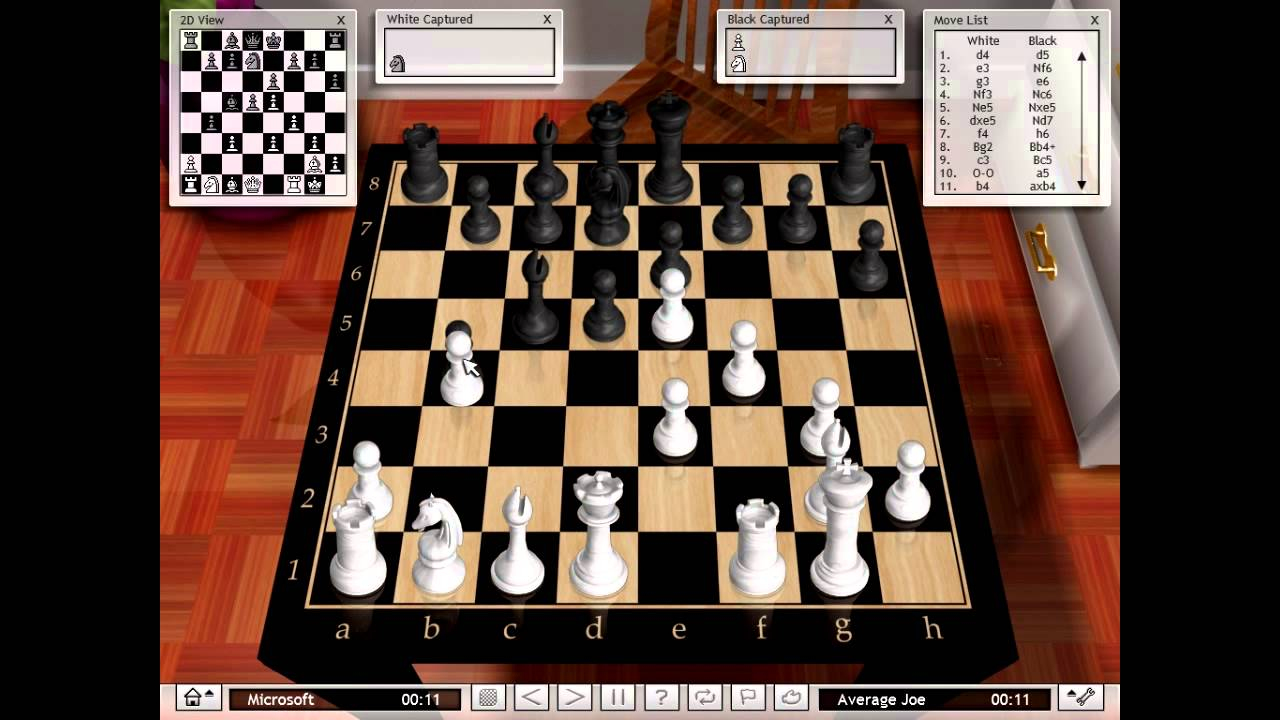
\includegraphics[scale=0.25]{chess1}
\end{figure}


\begin{figure}[!ht]
  \centering
	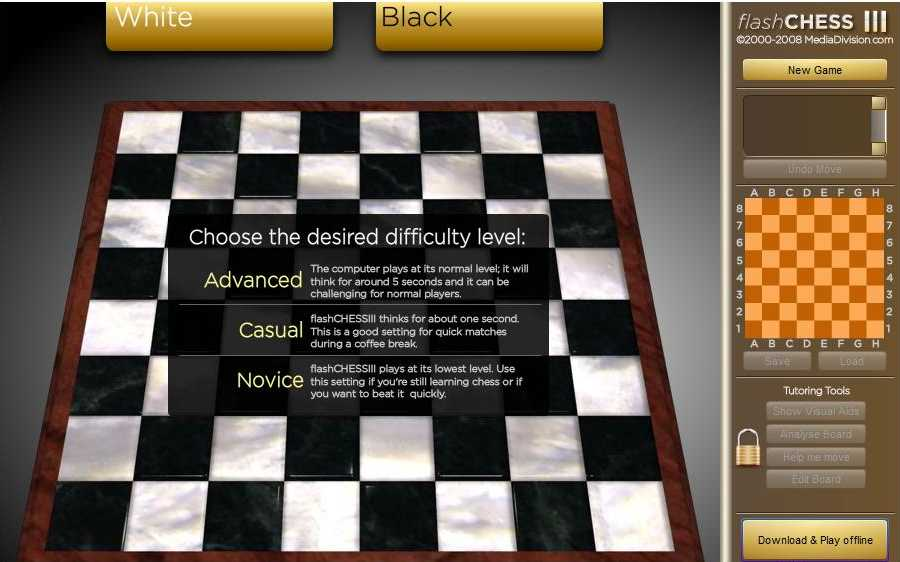
\includegraphics[scale=0.45]{chess2}
\end{figure}

\begin{figure}[!ht]
  \centering
	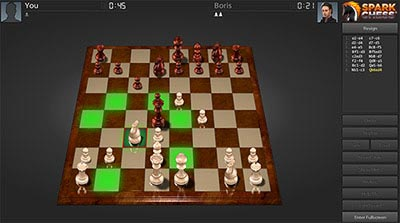
\includegraphics[scale=1]{chess4}
\end{figure}

\begin{figure}[!ht]
  \centering
	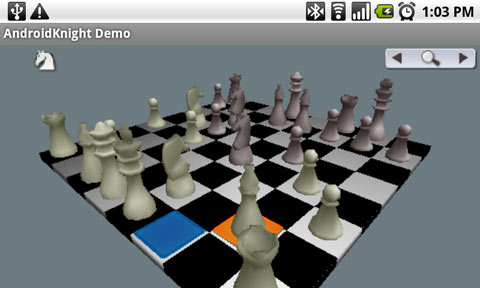
\includegraphics[scale=0.84]{chess5}
\end{figure}




\end{document}